% !TeX spellcheck = it_IT
\newpage
\section{Reti neurali profonde}
Sono algoritmi di apprendimento automatico per associare etichette a dati in ingresso. I dati attraversano la rete come vettori che ne sintetizzano le \textbf{feature}. Ogni strato si compone di neuroni che applicano una \textbf{funzione di attivazione} per modificare
\subsection{Lifecycle}
\subsubsection{Addestramento}
L'addestramento delle reti neurali avviene in maniera distribuita sfruttando server equipaggiati con GPU o TPU, che sono specifiche apposta per calcoli paralleli.\\
Può richiedere oltre un mese e una grossa quantità di energia.
\subsubsection{Dispiegamento}
I modelli addestrati sono poi distribuiti nei datacenter in modo che possano essere utilizzati dagli utenti finali.

\subsection{Consumi}
I fattori che influenzano i consumi sono:
\begin{itemize}
	\item L'\textbf{algoritmo} scelto, la sua \textit{implementazione}, il numero di \textit{parametri} e il \textit{tempo} di addestramento e di querying
	\item Il \textbf{numero di server} e \textbf{TPU/GPU} utilizzati per tutto il ciclo di vita e il \textit{PUE} dei datacenter in questione
	\item L'\textbf{intensità di anidride carbonica} equivalente del mix energetico in uso
\end{itemize}
\subsubsection{GPT-3}
Consideriamo come caso di studio GPT-3, un \textit{Large language model} del 2020 con 175 miliardi di parametri e allenato su 10.000 GPU.\\
Vediamo i dati:
\begin{itemize}
	\item \textbf{Addestramento} di 15 giorni:
	\begin{itemize}
		\item $10.000$ GPU Nvidia V100 ($300W$), produzione $150 kgCO_2-eq / GPU$
		\item $625$ server (potenza media $250W$), produzione $2.000 kgCO_2-eq/server$
		\item PUE $1.1$
		\item $\alpha_{USA}=0.400 kgCO_2-eq/kWh$
		\item $\tau=0.95$
	\end{itemize}
	\item \textbf{Dispiegamento} di $1.5$ anni:
	\begin{itemize}
		\item $3620$ server Nvidia HGX A100 ($250W$), produzione $2.000 kgCO_2-eq/server$
		\item PUE $1.1$
		\item $\alpha_{USA}=0.400 kgCO_2-eq/kWh$
		\item $\tau=0.95$
	\end{itemize}
\end{itemize}

Di seguito lo svolgimento:
\begin{enumerate}
	\item \textbf{Qual è l’impronta di anidride carbonica equivalente per la produzione dell’hardware?}
	Dati $H_t$ e $H_q$ l'insieme dell'HW necessario alle due fasi e $C_i(h)$ una funzione che restituisce per ogni componente HW le emissioni per la produzione:
	\begin{equation*}
		C_{tot}=\sum_{h \in H_t \cup H_q} C_i(h) = 2000 kg \cdot 625 + 150 kg \cdot 10000 + 2000 kg \cdot 3620 = 9990 tCO_2-eq
	\end{equation*}
	\item \textbf{Qual è il consumo energetico dovuto alla fase di addestramento?}
	Dati $t_j$ il tempo di addestramento, $\epsilon_j$ il PUE e $P_j$ la potenza media per ogni componente hardware nella fase di addestramento:
	\begin{equation*}
		E_t  = \sum_{j \in H_t} t_j \epsilon_j P_j \simeq \epsilon \sum_{j \in H_t} P_t \Delta T_t = 1.1 \cdot (10000 \cdot 300W + 625 \cdot 250W) \cdot 360h = 1250 MWh
	\end{equation*}
	\item \textbf{Qual è il consumo energetico dovuto alla fase di dispiegamento?}
	Dati $t_k$ il tempo di addestramento, $\epsilon_k$ il PUE e $P_k$ la potenza media per ogni componente hardware nella fase di dispiegamento:
	\begin{equation*}
		E_q  = \sum_{k \in H_q} t_k \epsilon_k P_k \simeq \epsilon \sum_{k \in H_q} P_q \Delta T_q = 1.1 \cdot 3620 \cdot 250W \cdot 24h \cdot 365 \cdot 1.5 \simeq 13081MWh
	\end{equation*}
	\item \textbf{Qual è l’impronta di anidride carbonica dovuta alla fase di addestramento?}
	\begin{equation*}
		C_t = \frac{E_t}{\tau}\cdot \alpha_{USA} = \frac{1250}{0.95}\cdot 10^3 kWh \cdot 0.400 \frac{kgCO_2-eq}{kWh}\simeq 526 tCO_2-eq
	\end{equation*}
	\item \textbf{Qual è l’impronta di anidride carbonica dovuta alla fase di dispiegamento?}
	\begin{equation*}
		C_q = \frac{E_q}{\tau}\cdot \alpha_{USA} = \frac{13080}{0.95}\cdot 10^3 kWh \cdot 0.400 \frac{kgCO_2-eq}{kWh}\simeq 5510 tCO_2-eq
	\end{equation*}
	\item \textbf{Quanto impatta l’addestramento sull’intero ciclo di vita?}
	L'intero ciclo di vita consuma:
	\begin{equation*}
		E = E_t + E_q = (1250 + 13081)kWh = 14331 kWh
	\end{equation*}
	e quindi l'addestramento corrisponde al $9\%$.\\
	Il totale di anidride carbonica equivalente:
	\begin{equation*}
		C = C_{emb}+C_t + C_q = (9990 + 526 + 5510)tCO_2-eq = 16026 tCO_2-eq
	\end{equation*}
	e quindi l'addestramento corrisponde al $3\%$.
\end{enumerate}
Concludendo, il grosso dei consumi corrisponde all'\textbf{embedded carbon} e alla fase di dispiegamento.
\subsection{Riduzione delle emissioni}
\subsubsection{Google 4M}
Google ha proposto quattro buone pratiche per rallentare e ridurre l'impronta delle reti neurali:
\begin{itemize}
	\item \textbf{Modelli}: l'uso di modelli più efficienti (\textit{sparsi} invece che \textit{densi})	può ridurre da 5 a 10 volte i calcoli necessari
	\item \textbf{Macchine}: l'uso di HW più efficiente può ridurre i consumi da 2W a 5W
	\item \textbf{Meccanizzazione}: l'uso di risorse Cloud può ridurre il consumo energetico da 1.4 a 2 volte
	\item \textbf{Mappa}: la scelta di un luogo con energia rinnovabile può ridurre le emissioni di $CO_2-eq$ da 5 a 10 volte
\end{itemize}
\begin{center}
	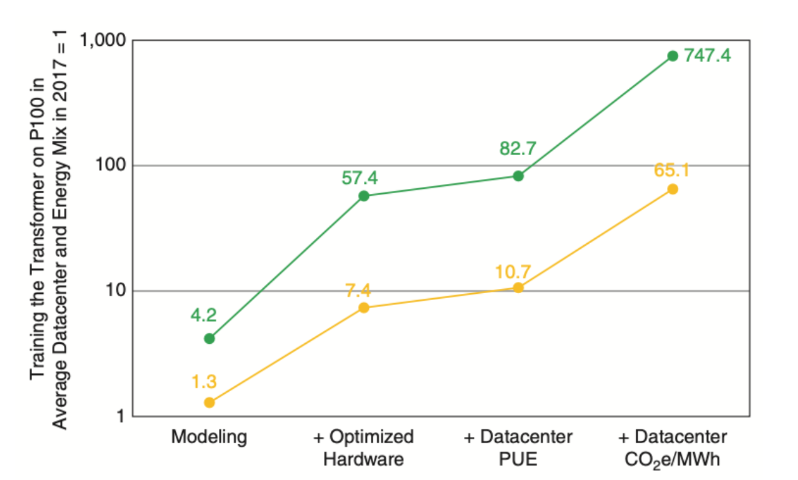
\includegraphics[scale=0.3]{4m.png}
\end{center}
Grazie alle 4M (e alle compensazioni di quote $CO_2$), nonostante l'energia totale utilizzata da Google sia aumentata negli ultimi 3 anni, la percentuale destinata al ML è rimasta stabile sotto al $15\%$, di cui $\frac{3}{5}$ dovuta al \textit{dispiegamento}.
\subsubsection{Modelli più efficienti}
Un esempio di modello più efficiente è \color{green}\textbf{GLaM}\color{black}, che nonostante abbia 7 volte i parametri di \color{red}GPT-3 \color{black} (essendo quindi più \textbf{accurato}), ne migliora anche l'\textbf{efficienza energetica}, anche grazie al fatto che è stato allenato in un datacenter con $\alpha=0.088 kgCO_2-eq/kWh$.
\begin{center}
	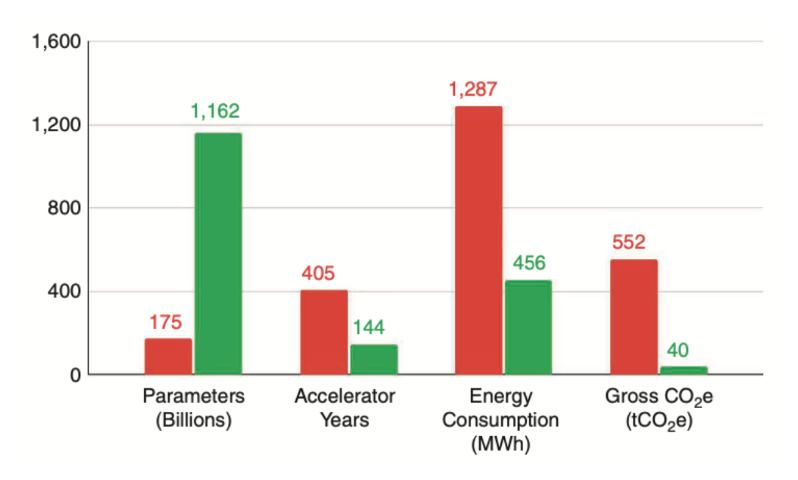
\includegraphics[scale=0.3]{glam.png}
\end{center}
\subsection{Conclusioni}
L'impatto delle reti neurali è elevato ma nelle Big Tech non supera comunque il $15\%$ dell'energia totale. La fase più costosa è quella di \textbf{dispiegamento} ($80\%-90\%$).\\
In ogni caso spesso i benefici portati alla società sono importanti e va quindi fatta un'analisi accurata del rapporto costi-benefici.